This master thesis is in context of a cooperation between the Visual Computing Institute at RWTH Aachen University and the Department of Oral and Maxillofacial Surgery (OMFS) at University Hospital RWTH Aachen (UHA).
The goal of this thesis is to simulate a virtual operating room for oral and maxillofacial surgeons in Virtual Reality (VR).
Workflows and procedures will be strongly oriented towards clinical practices of the oral and maxillofacial department in UHA.

Through the well established field of medical imaging, surgeons can get a very detailed view of patient’s specific anatomy and pathology today. 
It is an essential part of preparing for surgery.
Most common medical 3D image acquisition techniques (not exlusive) are computed tomography (CT), cone-beam computed tomography (CBCT) and magnetic resonance imaging (MRI).
CT / CBCT makes use of x-ray measurements from different angles to produce cross-sectional (tomographic) "slices" of the scanned site.
With this technique, bone structure and soft tissue can be displayed in medical imaging.
The disadvantage of these techniques is the exposure to carcinogenic x-rays.
In MRI, strong magnetic fields, magnetic field gradients and ultrasound are used to create tomography of the patients tissue.
Since this technique makes use of hydrogen atoms, which is predominantly present in patient's soft tissue, bone structure is not imaged well.
However, when studying mandibular joints for example, MRI is able to outperform CT \cite{RN65}.
The most recent one, CBCT, lowers radiation dosage of traditional CT and continually contributes to the accuracy of diagnostic tasks of the viscerocranium.
It is able to produce images with isotropic submillimeter spatial resolution, which is ideally suited for isolated viscerocranium scans. 
The radiation dosage of CBCT is less than traditional CT and thus helps optimize health-to-risk ratio \cite{WHITE2008689}.

As discussed, there are a variety of ways to acquire medical imaging.
However, the displaying methods of 3D medical imaging data is very limited for clinicians.
After acquiring raw data via mentioned techniques, volume images are generated. 
Generally, data is reconstruced in three planes (axial, sagittal and coronal).
Each plane is represented in "slices" which are 2D images of the volume image in an axis.
The distance between each slice can differ but is usually between one and five millimeters.

OMFS is very diverse. It has to handle a complex arrangement of bones, teeth, vessels, cartilage, nerves, muscles, skin and gland tissue.
These structures can be deeply complex, even more so in the viscerocranium.
Therefore, OMF surgeons rely heavily on accurate 3D medical imaging to plan procedures.
Even though three-dimensional objects are being analysed and also generated, they are viewed in a two-dimensional format on conventional computer screens.
The generated slices from medical imaging are viewed in the mentioned planes to get volumentric understanding of patient's underlying anatomy and pathology.
The problem with slices is that they are generally unsegmented and it is up to the viewer of the medical imaging to interpret them correctly.

To prepare for medical procedures, a number of preparational options are at the surgeons disposal.
Each of those common practices will be discussed based on how well it is suited for the individuality of patients, the realism and the cost (time and resources) associated with preparing for the operation.

The most common preparation technique is the mental simulation in which the surgeon uses his imagination to get a mental image of the surgical site.
This is solely dependant on the experience and spatial imagination of the surgeon. 
Hence it can be very patient specific, which is the goal in such an excercise.
The realism however is low to medium and the costs are also dependant on the expercience and skill of the surgeon himself.

Another, yet very costly technique is a simulation on 3D-printed models.
Since patient data is used here, it is an highly patient specific and highly realistic simulation.

In papersimulations, surgeons draw out treatment plans.
This is usually little patient specific and not realistic, however the costs are very low too.

The last technique presented are operational textbooks and videos.
They are not patient specific at all, but due to real operations being depicted the realism is generally low to medium.
The cost is also almost zero since the hospital will generally own a number of textbooks and videos for training.

Each of theses techniques has major disadvantages.
They all cannot actively reflect the underlying specific anatomy and pathology of the patient and lack spatial perception.
Also, the 3D medical imaging, which gets viewed on 2D computer screens, has to be translated back onto the patient via the surgeons imaginative power. 
As discussed, there does not seem to be a trivial technique which all surgeons should use.
Surgeons will often use a combination of mentioned techniques to get the best results.
In the preparation stage, it is crucial that the operator gets a well defined mental image by 3D medical imaging data of the patient's anatomy and pathology.

This thesis aims to improve medical imaging and pre-operational planning by using a modern approach with head-mounted displays.
By using acquired 3D medical imaging in a virtual reality application, a very patient specific, highly realistic and only moderately costly technique with which surgeons can prepare for operations is pursued.

This thesis aims to achieve the following advantages over conventional methods:
\begin{compactenum}[label=(\alph*)]
    \item Familiarize the operator with the patient specific anatomy and pathalogy before operating
    \item The ability to simulate important operation steps
    \item Allow revision of the virtual operation as often as needed
    \item Recording and analysis of users and others virtual operations
    \item Test out procedures
\end{compactenum}

Especially the imaging of voluminous objects is mentally demanding and this thesis hopes to eliminate this problem completely by providing realistic 3D medical imaging in virtual reality.
This thesis is part of an applied virtual and augmented reality workflow for oral and maxillofacial surgery using head mounted displays (HMDs) as described in Figure \ref{fig::ProjectPlan}.

\begin{figure}[ht!]
    \centering
    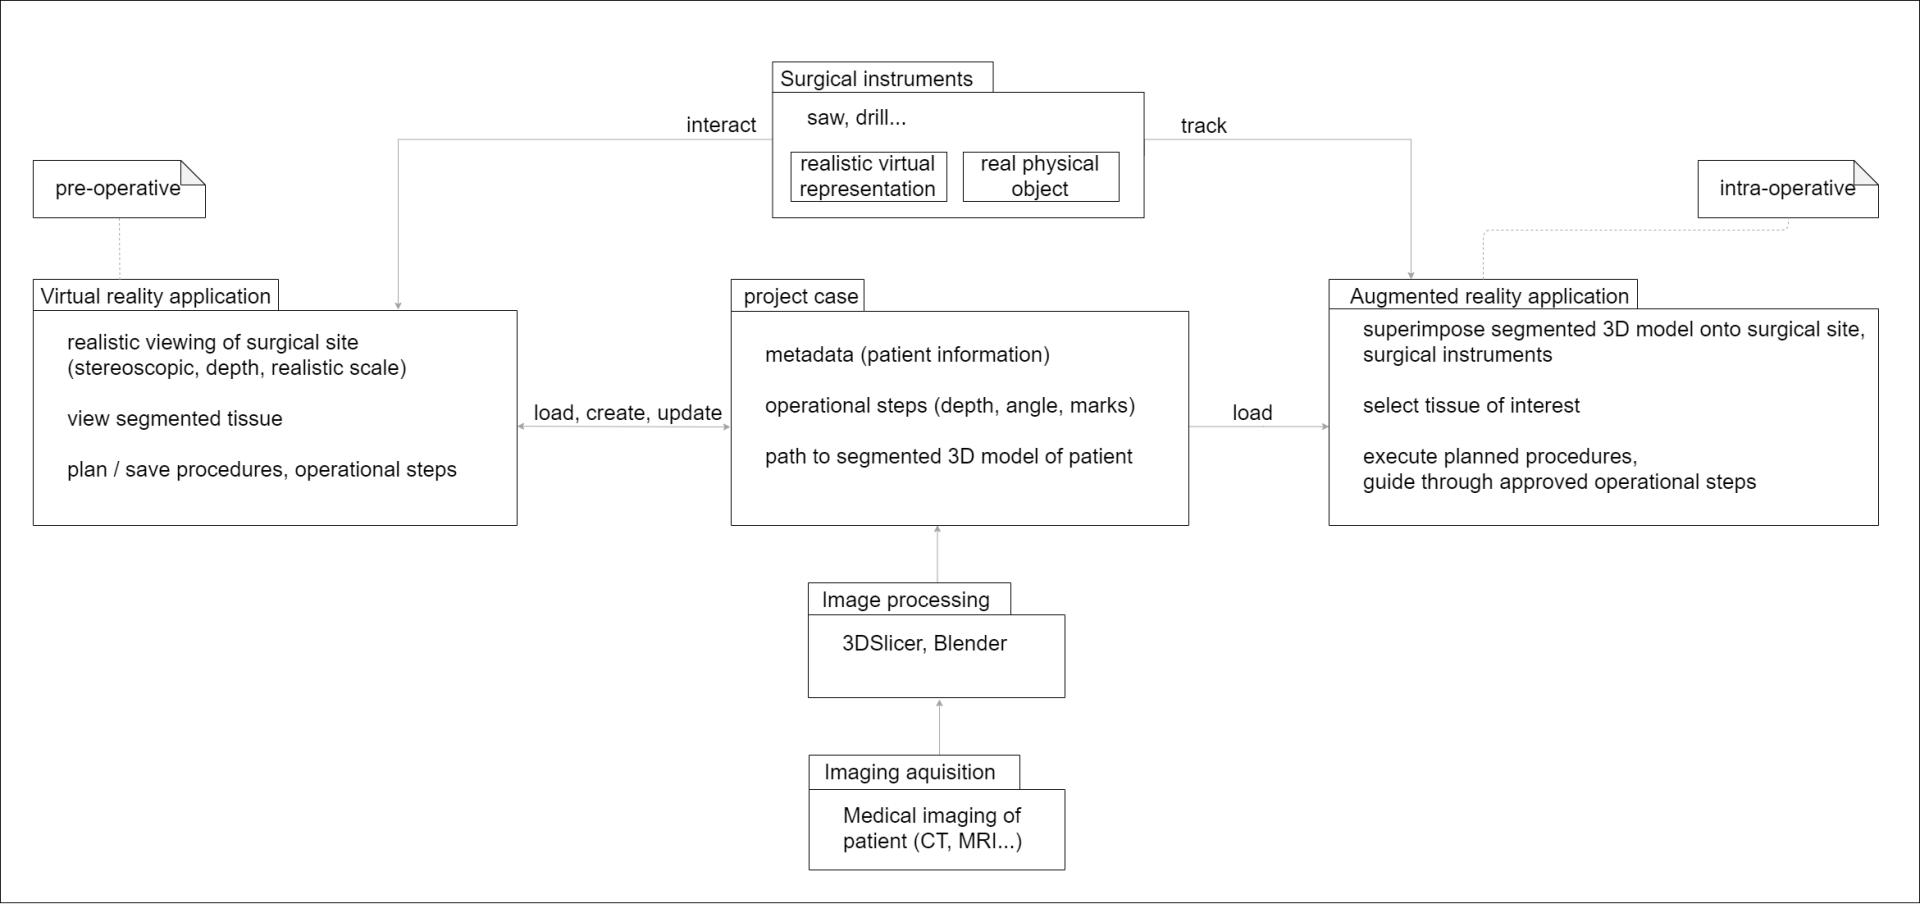
\includegraphics[width=\linewidth]{images/project_plan.png}
    \caption{\label{fig::ProjectPlan} Complete VR and AR workflow for surgeons concept}
\end{figure}

The main goal of this thesis is to create a pre-operative assistance tool in VR with HMDs for oral and maxillofacial surgery as highlighted in Figure \ref{fig::ProjectPlan}. 
In addition, the results of the pre-operative planning might be used intra-operatively to provide assistance via Augmented Reality (AR) as described in the workflow.
To provide a useful preparational tool, it is critical to simulate individual operation steps.
Planned steps will be storable in a format in which they can be loaded and viewed in both the virtual and augmented reality applications bi-directionally as described.
By planning the operational steps in virtual reality, planned procedures can easily be shown to other staff involved.
Naturally, it will be of uttermost importance that we have medical equipment and an appropriate virtual environment recreated remarkably close to reality.

The remainder of this Exposé is structured as follows: Chapter 2 provides a brief overview of related endevours made in the medical field.
Chapter 3 gives a scope of the thesis and a broad monthly schedule.